\documentclass[../thesis.tex]{subfiles}

\begin{document}

\begin{figure}
  \centering
  \begin{subfigure}[b]{0.3\linewidth}
    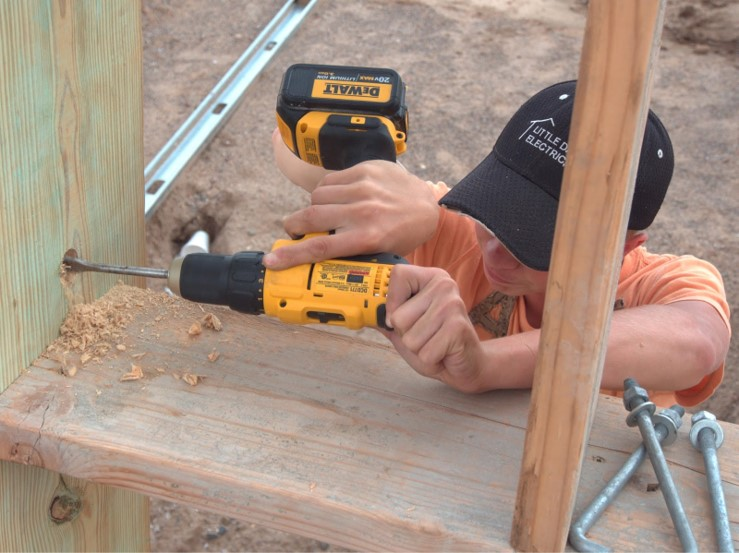
\includegraphics[width=\linewidth]{./Introduction/Drill.jpg}
  \end{subfigure}
  \hfill
  \begin{subfigure}[b]{0.3\linewidth}
    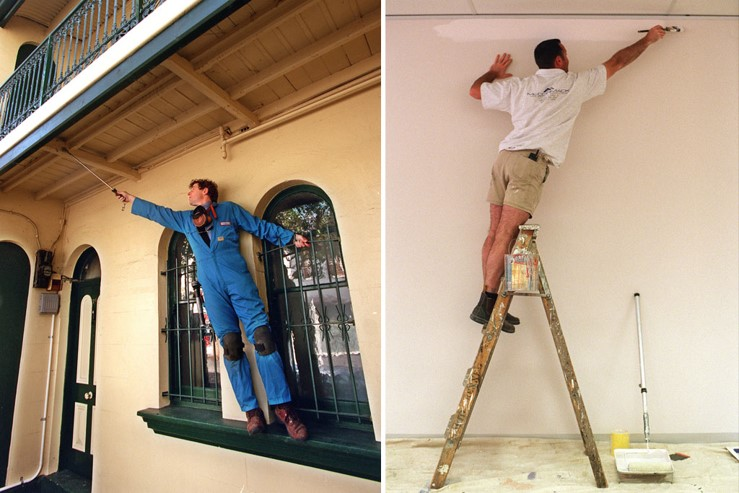
\includegraphics[width=\linewidth]{./Introduction/ladder.jpg}    
  \end{subfigure}
  \hfill
  \begin{subfigure}[b]{0.3\linewidth}
    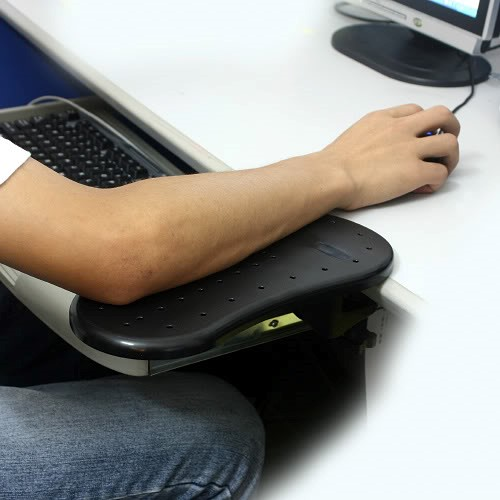
\includegraphics[width=\linewidth]{./Introduction/mouse.jpg}    
  \end{subfigure}
  \label{fig:HumanContact}
  \caption{Humans using contact to improve reach, accuracy, and stability}    
\end{figure}



Contacting the world can provide stability, support, and sensory information.
Humans benefit from touching the world in situations from blindly detecting an object in the back of the refrigerator, to leaning on a stair railing. 
In the recent DARPA robotics challenge top robotics research teams from around the world submitted robots to attempt an obstacle course of challenges.
Many of these robots fell on the stairs. 
Not a single robot used the railing \cite{Atkeson2015}.
Even drunk people know to use railings, so there is plenty of room for improvement in robotics.

However, in robotics there are good reasons to avoid contact with the environment.
Hitting the world can provide large forces that destabilize or break the robot.
Relying on contacts can be dangerous as slight alterations in the world or errors in robot position may drastically alter the contact forces.
Instead of firmly grasping a handle, a few centimeters of error have caused robots to embarrassingly grasp air and fall over.
%% \cite{DarpaRoboticsVideo}.
Even when working entirely in simulation contacts between rigid bodies cause problems for physics engines.


Contacts introduce non-smooth discontinuities, which presents a challenge for many tools in the roboticists arsenal.
The benefits of contacts occur on a measure-zero manifold in the robot's configuration space.
For example, hand rests comfortably on a table at a specific configuration of shoulder, elbow, and wrist positions.
A slight extension of the elbow while fixing all other joints leads to the hand puncturing the table, while a slight contractions pulls the hand into the air and the table might as well not exist.
Random sampling and gradient decent are two techniques that appear in the solution to many robotics challenges, but both have difficulty with these measure-zero contact manifolds.
This thesis explores and extends techniques of sampling based and gradient methods to the problems of localization and planning, with the addition of contact forces and measurements.


%% Standard numerical techniques of discretization fail to capture the near instantaneous effects of contact both in modeling uncertainty and planning.


\section{Motivation}
My personal motivation for the topics covered in this thesis come, in part, from my past experience as a robotics engineering building robots that build airplanes.
Currently, large robotic arms equipped with expensive, specialized end effectors perform a variety of tasks for aerospace manufacturing, including drilling holes, inserting fasteners, milling, carbon fiber placement and layup, and sealant application.
While there are many potential directions of research to improve these already impressive machines, two striking issues are addressed by my work.

\subsection{Jigs are More Expensive Than Robots}

\begin{figure}
  \centering
  \begin{subfigure}[b]{0.586\linewidth}
    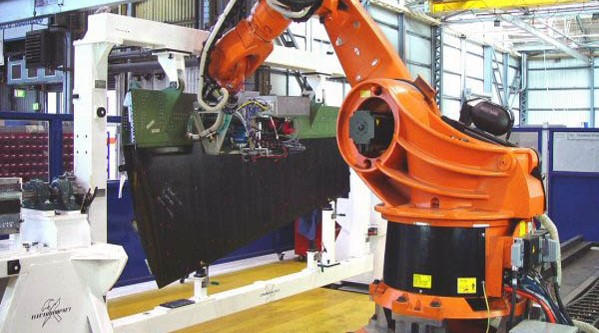
\includegraphics[width=\linewidth]{./Introduction/Robot1Outside.jpg}    
  \end{subfigure}
  \hfill
  \begin{subfigure}[b]{0.4\linewidth}
    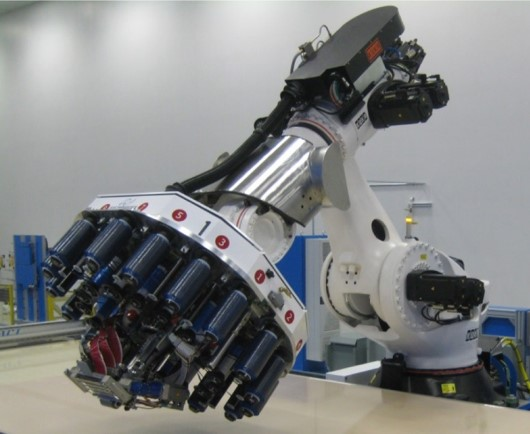
\includegraphics[width=\linewidth]{./Introduction/Robot2Outside.jpg}    
  \end{subfigure}
  \label{fig:KukaRobots}
  \caption{Robots working on the outside of parts held firmly in jigs}
\end{figure}

Robots that perform one type of task on one section of an airplane can cost millions of dollars.
However the jig that holds the airplane section while the robot works can cost more than the robot.
These jigs may have more actuators and tighter tolerances than the robotic system.
When the robot begins work on a new section, before ever making a measurement the jig has already located the part to within a few inches.
A few scripted measurement with a probe, programmed by an engineer, are sufficient to fully localize the part to within the needed tolerances.
%% These high costs and skilled engineering time are only acceptable because the expense is amortized over many
When amortized over many airplanes the per-part cost drops.
However, this process is inflexible and poorly suited to low-rate manufacturing.

If the robot could localize the part from a wide range of part configurations, and if the robot could reason about internal assembly tolerances then jigs could be make more cheaply, robots would become more versatile, less part-specific programming would be required, and machining accuracy could improve.

\subsection{Robots Stay on the Outside}

\begin{figure}
  \centering
  \label{fig:PeopleInWing}
  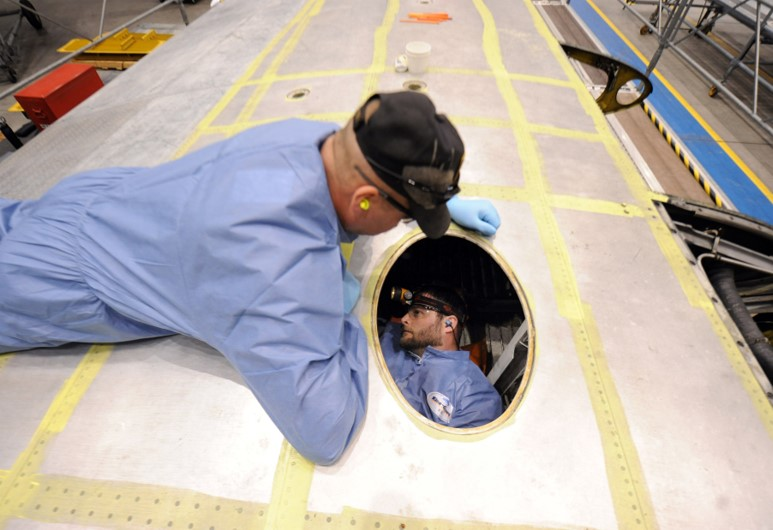
\includegraphics[width=.7\linewidth]{./Introduction/PeopleInWing.jpg}  
  \caption{Workers crawling in the confined spaces of an airplane wing}
\end{figure}

Large robotic arms cannot fit in the confined spaces of an aircraft.
While a team of people may include workers on both the inside and outside, large robots are limited to just the outside.



\section{Approach}
The work in this thesis address two separate problems. The first is the task of localizing an object through measurements made using contact measurement.
The second is the task of planning a trajectory for a robotic arm that is too long to support its own cantilevered weight, and so must rest on the environment for support.
Unifying the two problems is the challenges associated with contacts.

\subsection{Localization}

\begin{figure}
\centering
    \begin{subfigure}[b]{.49\linewidth}
      \includegraphics[width=\linewidth, clip, trim=9in 3in 0in 1in]{./Introduction/Overview2}
        \caption{}
        \label{fig:Rigid:Overview_1}
    \end{subfigure}
    \hfill
    \begin{subfigure}[b]{.49\linewidth}
      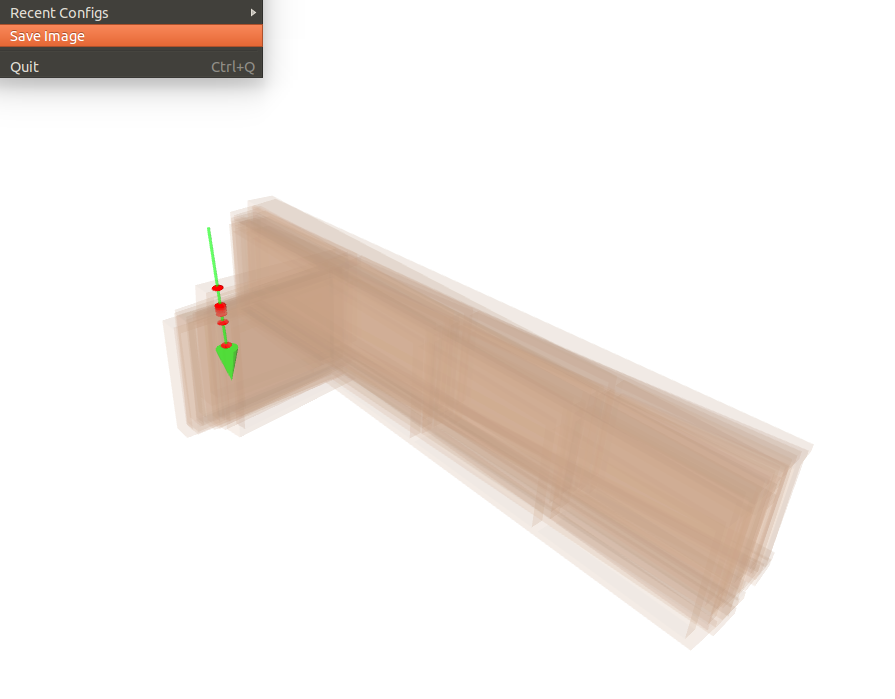
\includegraphics[width=\linewidth, clip, trim=1.5in 1.5in 1.5in 1.3in]{./Introduction/Particle_Intersection}
        \caption{}
        \label{fig:Rigid:Overview_2}
    \end{subfigure}
%% \includegraphics[width=2.5in, clip, trim=9in 3in 0in 1in]{Overview2}
%% \includegraphics[width=2.5in, clip, trim=0in 4in 12in 2in]{Overview2}
\caption{\subcap{fig:Rigid:Overview_1}: The robot performing a touch measurement}\\
\subcap{fig:Rigid:Overview_2}: The belief of the part location and measurement
\label{fig:Rigid:Overview}
\end{figure}

In the localization task the robot must estimate the pose $X$ of an object based on a set of measurements $Z_t = \{z_1, ..., z_t\}$ made by probing the object.
The robot chooses where to probe, and the measurements are a function of the object and chosen measurement action.
A triangular mesh describes the object geometry and a frame is attached to this mesh. 
The state $X$ is the $SE(3)$ transformation from a fixed world frame to this part frame. 
This is a 6-dimensional state stored as position $(x,y,z)$ and orientation angles $(\alpha, \beta, \gamma)$. 
Initially it is assumed the geometry is rigid, thus the state can be fully described as the $SE(3)$ configuration of a frame attached to the part \ref{sec:rigid_body}.
Later, this is generalized to parts with internal uncertainty \ref{sec:datum}.
A further assume is that the part is fixed in space relative to a world frame and that probing actions do not perturb the state. 

Rather than calculating a single best estimate of the pose, a probability distribution represents the uncertainty in knowledge.
Estimating the probability distribution is important both for choosing effective measurements and knowing when the part is localized sufficiently. 
For feasibility, this probabilistic belief is represented numerically by a list of points drawn from the true distribution called \textit{particles}. 
A measurement updates the belief using a \textit{particle filter} \cite{Thrun2000a}.

However particle filters behave poorly both when the dimensionallity of the system grows large and when measurements become precise \cite{Koval2013}. 
In the problems considered there is a large initial uncertainty, and achieving high tolerance performance necessitates measurements with low uncertainty.
Updating the belief after performing such a measurement will eliminate most particles, leaving a poor representation of the posterior. This problem is called particle starvation.

This thesis first presents a solution to particle starvation during touch localization (section \ref{sec:rigid_body}) using a particle filter with an alternate update procedure that is able to combine accurate measurements with the prior. 
This particle filter is then generalized to parts with internal uncertainty (section \ref{sec:datum}).

To minimize the time taken to localize the part, the robot should choose informative measurement actions.
To achieve this, many actions are sampled and the one with the highest expected \textit{information gain} is selected. 
Fully predicting this is also computationally expensive, thus previous methods using this metric introduce delays during which the robot pauses between measurements and yet still only samples a small number of actions.
This approach involves a fast approximation for information gain that takes advantage of the discretized belief from the particle filter (section \ref{sec:information gain}). 
This enables the sampling hundreds of potential measurement actions in a few seconds. 



%% At any time step we have a belief of the state $bel(x_t) = p(x_t| Z_t)$. 
%% Measurements are a non-linear probabilistic function of the true state: $z_t \sim p(z_t|X)$. 
%% As in all Bayesian filters, the belief $bel(x_{t+1})$ is calculated recursively as follows \footnote{The full update of a Bayesian filter also includes a process model. Our assumption of a fixed part yields the static process model and this simpler formulation}:
%% \begin{align}
%% bel(x_{t+1}) \leftarrow \eta \ p(z_t|x_t) \  bel(x_t)
%% \end{align}
%% with $\eta$ as a normalization factor. Each new measurement value triggers an update to the belief $bel(x)$. 

Figure \ref{fig:Rigid:Overview} shows the experimental setup.
A 7-DOF robotic arm equipped with a touch probe performs measurements on an object \subcap{fig:Rigid:Overview_1}.
These measurements are used to update the belief \subcap{fig:Rigid:Overview_2}. The belief is the used to determine good information gathering future measurement actions.


\subsection{Motion Planning}
The motion planning task considered here involves planning trajectories for a robotic arm through an environment.
The robot arm begins at initial joint angles and the goal is to apply torques on the joints to move the end effector of the robot to some specified location in the workspace.
When planning, the robot arm kinematics and dynamics, joint torque limits, and the environment are known.
Of particular interest is the dynamics model, as it models contact forces at specified locations on the robot.

When not in contact with the environment the robot dynamics obey the manipulator arm equation \cite{murray1994mathematical}.
However, when in contact, additional forces are applied to the arm obeying a spring model: The force is proportional to the penetration distance, in the direction pushing the arm out of the environment.
To maintain stability in the model, the simulated environment is kept squishy with a spring constant significantly lower than the physical reality.

In the tasks considered in this thesis, the robot is not capable of reaching the goal point without using contact points, thus the motion planner must make use of contacts.
To ensure this the arm used is long and thin, the torque limit is low, and goal positions are chosen far from the base of the arm.
Thus the motors alone are not able to overcome the weight of the cantilevered robot arm.

Two approaches are used to plan: trajectory optimization and a sample-based planner.
In the trajectory optimization framework a function determines the cost of a trajectory, and an initial trajectory is iteratively improved using gradient descent until a local optimum is achieved.
The obvious choice for a cost function would penalize not reaching the goal and penalize joint torques, either through soft or hard constraints.
However due to the local nature of contacts, potentially useful contacts that are not yet made have no influence on the cost function, and these solutions will never be discovered.
The solution is an augmentation of the dynamics model, allowing contact forces at a distance.
This provides a much better conditioned cost function, at the expense of accurately modeling the world.
Towards the end of optimization the model parameters are altered to enforce a realistic solution.

When initialized well, this optimization approach produces trajectories that keep joint torques low by making and breaking contacts.
However, the cost function is still littered with non-optimal local minima, and escaping these proves difficult.
Thus a sampled based planner is employed to generate trajectories that can either directly be used, or that serve as a decent initialization for the optimization approach.
Again the thin contact manifold presents problems.
Sampled based planners rely on generating trajectories to connect probabilistically sampled configurations, but the thin contact manifold renders naive approaches useless.
The solution used augments the extension function of a sampled based planner, causing extensions to make progress towards their goal while staying on the contact manifold as necessary.



\end{document}
